\documentclass[pdflatex,sn-mathphys-num]{sn-jnl}

\usepackage{graphicx}
\usepackage{booktabs}
\usepackage{amsmath,amssymb}
\usepackage{tikz}
\usetikzlibrary{arrows.meta,positioning}
\usepackage{xcolor}
\usepackage{listings}

\setlength{\textfloatsep}{8pt plus 2pt minus 2pt}
\setlength{\intextsep}{6pt plus 2pt minus 2pt}
\setlength{\abovecaptionskip}{4pt}
\setlength{\belowcaptionskip}{2pt}

% Strongly discourage breaking words with hyphens at line ends; let
% word-spacing absorb the slack instead, falling back to a hyphen
% only where truly unavoidable (e.g. long code listings).
\hyphenpenalty=5000
\exhyphenpenalty=3000
\emergencystretch=3em

\lstset{
  basicstyle=\ttfamily\footnotesize,
  columns=fullflexible,
  keywordstyle=\color{teal!70!black},
  commentstyle=\color{green!45!black},
  stringstyle=\color{purple!60!black},
  breaklines=true,
  frame=single,
  framesep=3pt,
  backgroundcolor=\color{gray!5},
  showstringspaces=false
}

\raggedbottom

\begin{document}

\title[Enhanced IoT Healthcare Monitoring for Obese Adults]{An Enhanced IoT-Based Healthcare Monitoring System for Obese Adults}

\author*[1]{\fnm{Lahcen} \sur{Atti}}\email{atti.lahcen@gmail.com}

\author[1]{\fnm{Mohamed} \sur{Saber}}\email{mohamed.saber@edu.uiz.ac.ma}

\author[1]{\fnm{Nacer} \sur{Boubkraoui}}\email{n.boubkraoui@uiz.ac.ma}

\author[1]{\fnm{Mouhamed} \sur{Dib}}\email{m.dib@uiz.ac.ma}

\author[1]{\fnm{Hassan} \sur{Ouahi}}\email{h.ouahi@uiz.ac.ma}

\affil*[1]{\orgdiv{Faculty of Applied Sciences -- Ait Melloul}, \orgname{Ibn Zohr University}, \orgaddress{\city{Ait Melloul}, \country{Morocco}}}

%%-----------------------------------------------------------------%%
\abstract{This paper presents an enhanced Internet-of-Things (IoT)
healthcare monitoring prototype for obese adults, inspired by the
work of Gupta et al.~\cite{gupta2020}. The prototype combines a
DS18B20 digital ambient-temperature probe, a MAX30102
pulse-oximeter/heart-rate sensor, and a dual-core ESP32
microcontroller behind a patient-authenticated on-device menu,
publishing telemetry over MQTT to a ThingsBoard cloud dashboard.
Relative to the baseline platform, the system improves
ambient-temperature sensing accuracy ($\pm0.1\,^\circ$C vs.\
$\pm0.5\,^\circ$C), replaces an 8-bit microcontroller and unencrypted
HTTP transport with a Wi-Fi-capable ESP32 and MQTT, and moves from a
proprietary paid cloud subscription to an open-source dashboard. A
companion Android application concept for multi-patient dashboards
and threshold-based alerting is also described. This paper reports
the hardware design, firmware architecture, and cloud integration of
the prototype; clinical validation against a reference instrument is
identified as future work.}

\keywords{IoT, Healthcare monitoring, Obesity, ESP32, MQTT, ThingsBoard}

\maketitle

%%-----------------------------------------------------------------%%
\section{Introduction}\label{sec:intro}

Obesity affects over 650 million adults worldwide and increases the
risk of cardiovascular and metabolic complications~\cite{who2023}.
Continuous monitoring of vital signs -- blood-oxygen saturation
(SpO\textsubscript{2}) and heart rate -- together with ambient
temperature logging can support early detection of complications, but
commercial remote patient monitoring (RPM) devices remain
cost-prohibitive for many deployments. This paper
presents a low-cost IoT-based monitoring prototype for obese adults
that builds on the platform proposed by Gupta et
al.~\cite{gupta2020}. Relative to that baseline, four improvements are
targeted:

\begin{itemize}
  \item higher-accuracy digital temperature sensing
    ($\pm0.1\,^\circ$C vs.\ $\pm0.5\,^\circ$C);
  \item MQTT-based telemetry in place of unencrypted HTTP polling;
  \item an open-source ThingsBoard cloud dashboard in place of a
    proprietary subscription service;
  \item a rechargeable Li-ion power supply in place of a fixed
    12\,V DC adapter.
\end{itemize}

This paper makes the following contributions:
\begin{enumerate}
  \item A hardware and firmware redesign of the baseline platform
    using an ESP32 microcontroller, a DS18B20 digital thermometer,
    and a MAX30102 pulse oximeter, with an on-device
    patient-login menu (Sect.~\ref{sec:design}).
  \item An MQTT/ThingsBoard cloud-integration layer with a defined
    topic hierarchy and JSON telemetry schema
    (Sect.~\ref{sec:mqtt}).
  \item A concept design for a multi-patient Android dashboard
    application with threshold-based alerting
    (Sect.~\ref{sec:mobile}).
\end{enumerate}

%%-----------------------------------------------------------------%%
\section{Related Work}\label{sec:related}

The baseline platform proposed by Gupta et al.~\cite{gupta2020}
combines an Arduino ATmega328 microcontroller, an LM35 analogue
temperature sensor ($\pm0.5\,^\circ$C), a wrist-worn blood-pressure
cuff, and unencrypted HTTP transmission to a proprietary cloud service
(iotgecko.com). It established feasibility for obesity-focused
wearable monitoring, but four limitations motivate the present work:
(i)~the 8-bit AVR core has no native wireless connectivity and
requires an external radio module; (ii)~the analogue thermometry
chain is limited to $\pm0.5\,^\circ$C accuracy by ADC quantisation
noise; (iii)~HTTP transmission carries no transport-layer encryption;
and (iv)~the cloud subscription incurs recurring licensing cost around
a closed dashboard.

\begin{table}[!ht]
\caption{Baseline vs.\ enhanced platform (component-level comparison).}\label{tab:compare}
\centering
\begin{tabular}{@{}lll@{}}
\toprule
\textbf{Feature} & \textbf{Baseline~\cite{gupta2020}} & \textbf{This work}\\
\midrule
Microcontroller     & Arduino ATmega328     & ESP32 (dual-core, Wi-Fi/BLE)\\
Temperature sensor   & LM35 ($\pm0.5\,^\circ$C) & DS18B20 ($\pm0.1\,^\circ$C)\\
Cloud platform       & iotgecko.com (proprietary) & ThingsBoard (open-source)\\
Transport             & HTTP (unencrypted)     & MQTT\footnotemark[1]\\
Power source          & 12\,V DC adapter       & Li-ion battery ($\sim$8\,h)\\
BP sensing             & Wrist cuff              & Clinical arm cuff\footnotemark[2]\\
\botrule
\end{tabular}
\footnotetext[1]{The demonstrated prototype uses the MQTT broker's
  default unencrypted listener for development; TLS on the broker's
  secure port is the intended production configuration
  (Sect.~\ref{sec:mqtt}).}
\footnotetext[2]{Hardware slot present on the board design; firmware
  integration is future work (Sect.~\ref{sec:future}).}
\end{table}

%%-----------------------------------------------------------------%%
\section{System Design}\label{sec:design}

\subsection{Hardware Architecture}

Figure~\ref{fig:arch} shows the end-to-end data path. The
microcontroller is an ESP32-WROOM-32D development board (dual-core
Xtensa LX6, integrated Wi-Fi/BLE), replacing the Arduino ATmega328 and
its external wireless module. Ambient temperature is sampled by a
DS18B20 waterproof digital probe over a 1-Wire bus, removing the ADC
quantisation noise of the baseline's analogue LM35 chain. SpO\textsubscript{2}
and heart rate are sampled by a MAX30102 pulse-oximeter module over
I\textsuperscript{2}C, accessed through a MAX30100-compatible
pulse-oximeter driver library. A four-button matrix keypad and a
20$\times$4 character I\textsuperscript{2}C LCD provide local patient
interaction (DS18B20 data line on GPIO4; keypad keys~1--4 on GPIO27,
GPIO26, GPIO12, and GPIO14; LCD at I\textsuperscript{2}C address
0x27).

\begin{figure}[!ht]
\centering
\resizebox{0.98\linewidth}{!}{%
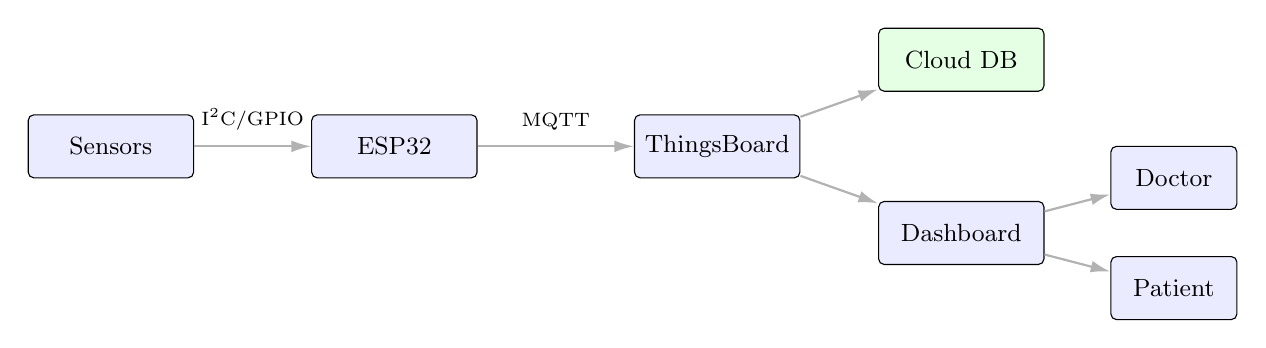
\begin{tikzpicture}[
  font=\small,
  every node/.style={align=center},
  box/.style={draw, rounded corners=2pt, fill=blue!8,
              minimum width=2.1cm, minimum height=0.8cm},
  cloudbox/.style={draw, rounded corners=2pt, fill=green!10,
                   minimum width=2.1cm, minimum height=0.8cm},
  arr/.style={-{Latex[length=2.5mm,width=1.5mm]}, thick, draw=gray!60}
]
\node[box] (sensors) at (0,0) {Sensors};
\node[box] (esp32) at (3.6,0) {ESP32};
\node[box] (tb) at (7.7,0) {ThingsBoard};
\node[cloudbox] (cloud) at (10.8,1.1) {Cloud DB};
\node[box] (dash) at (10.8,-1.1) {Dashboard};
\node[box, minimum width=1.6cm] (doctor) at (13.5,-0.4) {Doctor};
\node[box, minimum width=1.6cm] (patient) at (13.5,-1.8) {Patient};

\draw[arr] (sensors) -- node[above,yshift=2pt,font=\scriptsize]{I\textsuperscript{2}C/GPIO} (esp32);
\draw[arr] (esp32) -- node[above,yshift=2pt,font=\scriptsize]{MQTT} (tb);
\draw[arr] (tb) -- (cloud);
\draw[arr] (tb) -- (dash);
\draw[arr] (dash) -- (doctor);
\draw[arr] (dash) -- (patient);
\end{tikzpicture}%
}
\caption{System architecture: on-board sensors feed the ESP32, which
publishes MQTT telemetry to ThingsBoard; the cloud dashboard is
consumed by clinicians and patients.}\label{fig:arch}
\end{figure}

\begin{figure}[!ht]
\centering
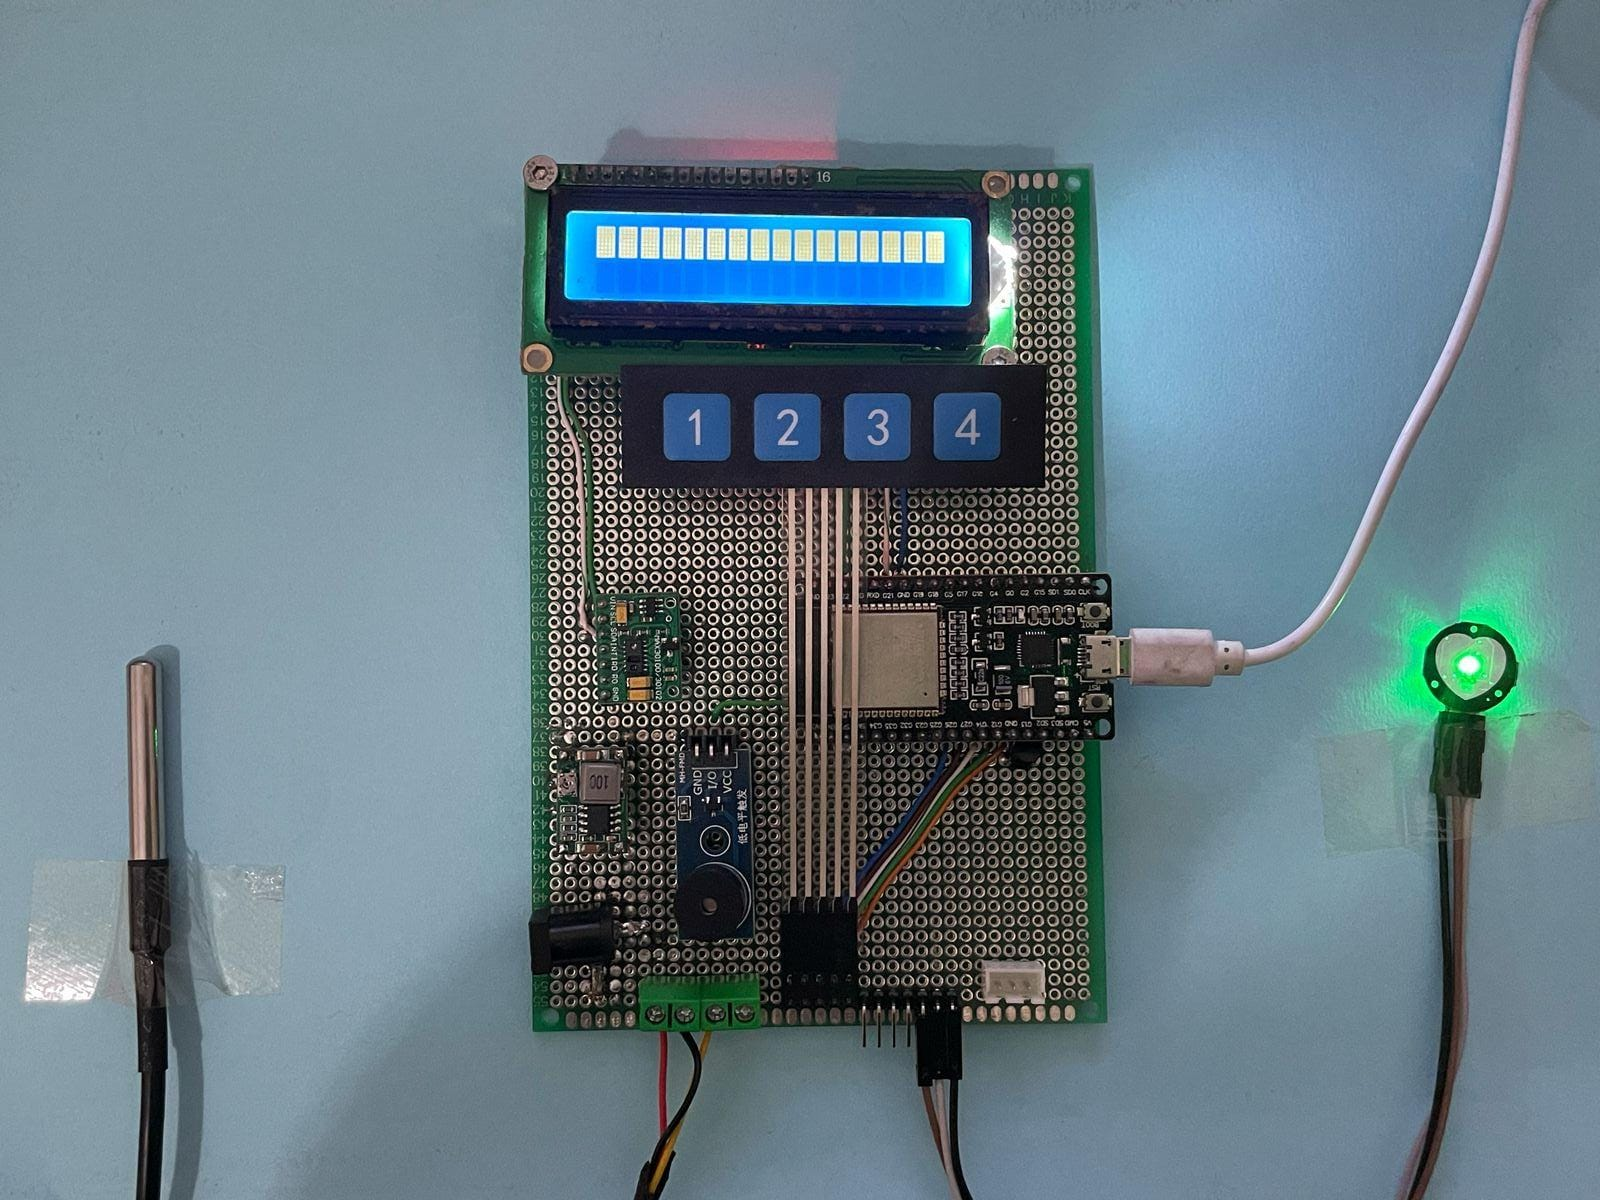
\includegraphics[width=0.6\linewidth]{images/fig-prototype.jpg}
\caption{Assembled prototype: LCD, keypad, ESP32, DS18B20 ambient
temperature probe, and MAX30102 pulse-oximeter sensor.}\label{fig:prototype}
\end{figure}

\subsection{Firmware Architecture}

The firmware implements a menu-driven state machine, shown live on
the on-device LCD in Fig.~\ref{fig:menu}. On boot, the patient must
enter a 4-digit code on the keypad before any measurement is
available; a successful verification unlocks the main menu
(Fig.~\ref{fig:menu}a), from which the patient selects
SpO\textsubscript{2}, heart rate (BPM), temperature, or data transfer.
Each measurement runs as a non-blocking 5-second state
(Fig.~\ref{fig:menu}b) so that the pulse-oximeter driver
(\texttt{pox.update()}) and keypad polling continue to execute during
the on-screen countdown animation, rather than blocking on a fixed
\texttt{delay()}, before the result is displayed
(Fig.~\ref{fig:menu}c). On ``Data Transfer'', the device assembles a
JSON payload from the most recent readings and publishes it to the
cloud (Sect.~\ref{sec:mqtt}).

\begin{figure}[!ht]
\centering
\begin{minipage}{0.32\linewidth}
\centering
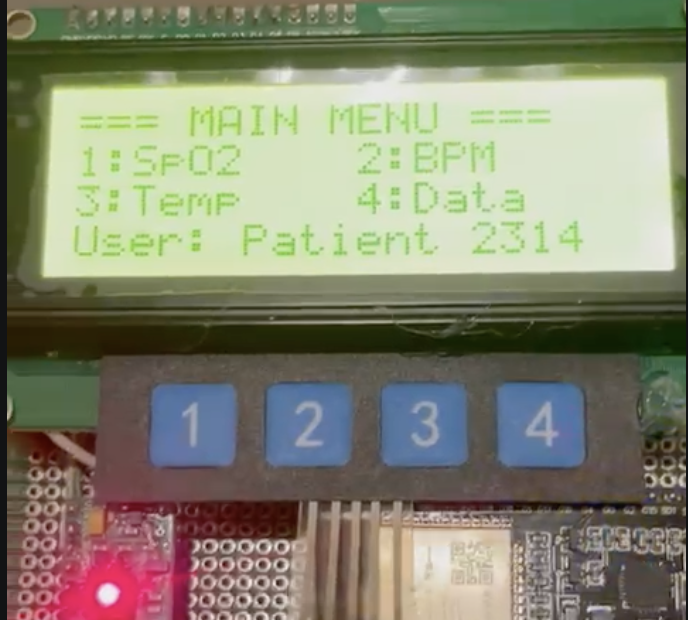
\includegraphics[width=\linewidth]{images/fig-menu-main.png}\\
\footnotesize (a) Main menu
\end{minipage}\hfill
\begin{minipage}{0.32\linewidth}
\centering
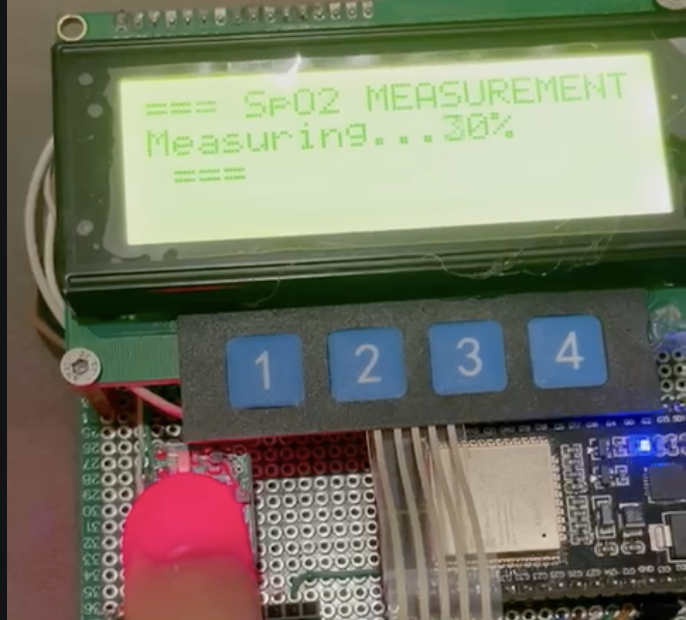
\includegraphics[width=\linewidth]{images/fig-spo2-measuring.png}\\
\footnotesize (b) SpO\textsubscript{2} measuring
\end{minipage}\hfill
\begin{minipage}{0.32\linewidth}
\centering
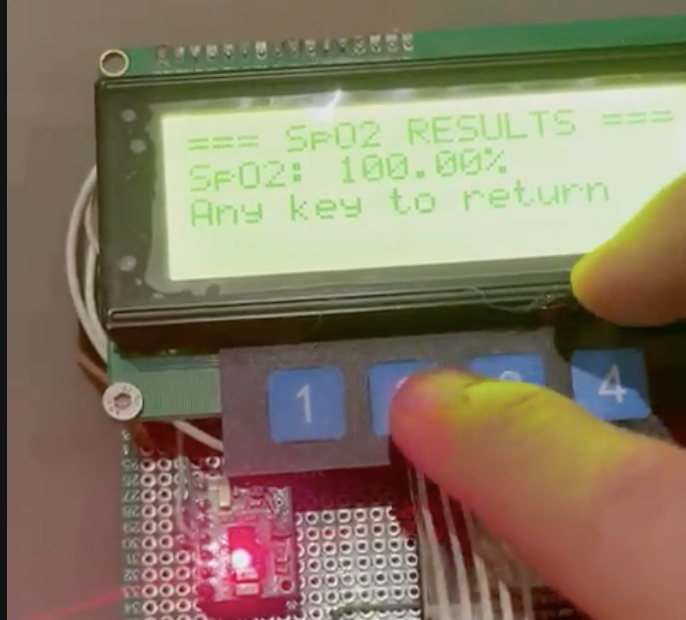
\includegraphics[width=\linewidth]{images/fig-spo2-result.png}\\
\footnotesize (c) SpO\textsubscript{2} result
\end{minipage}
\caption{On-device LCD menu, captured live: (a) main menu after
patient login, (b) non-blocking SpO\textsubscript{2} measurement in
progress, (c) SpO\textsubscript{2} result screen.}\label{fig:menu}
\end{figure}

Wi-Fi and MQTT broker credentials are configured at startup (Listing
1); the device token and network credentials shown here are
anonymised.

\begin{lstlisting}[caption={Wi-Fi and MQTT configuration (credentials anonymised).}]
// Wi-Fi credentials
const char* ssid     = "ANONYMIZED_SSID";
const char* password = "ANONYMIZED_PASSWORD";

// MQTT broker (ThingsBoard server)
const char* mqtt_server    = "demo.thingsboard.io";
const int   mqtt_port      = 1883;
const char* mqtt_client_id = "ESP32_Client";
const char* mqtt_username  = "ANONYMIZED_DEVICE_TOKEN"; // ThingsBoard device token
\end{lstlisting}

%%-----------------------------------------------------------------%%
\section{Cloud Connectivity and MQTT Implementation}\label{sec:mqtt}

\subsection{Telemetry Path}

On ``Data Transfer'', the firmware builds a JSON object from the
patient code and the most recent SpO\textsubscript{2}, heart-rate, and
temperature readings, and publishes it on ThingsBoard's fixed device
telemetry topic (Listing 2).

\begin{lstlisting}[caption={JSON payload construction and MQTT publish (device firmware).}]
String payload = "{";
payload += "\"patient_id\": \"" + patientCode + "\",";
payload += "\"SpO2\": " + String(oldSpO2) + ",";
payload += "\"BPM\": " + String(oldBPM) + ",";
payload += "\"Temperature\": " + String(oldTemp);
payload += "}";

client.publish("v1/devices/me/telemetry", payload.c_str());
\end{lstlisting}

The device authenticates to the broker using its ThingsBoard access
token as the MQTT username, following ThingsBoard's standard
device-token authentication scheme~\cite{thingsboard}. The
demonstrated prototype connects to the public demo broker
(\texttt{demo.thingsboard.io}) on its default unencrypted port 1883
for development; the broker's TLS listener on port 8883, with the
same token-based authentication, is the intended configuration for a
production deployment.

\subsection{Why ThingsBoard}

ThingsBoard was selected over commercial alternatives (e.g.\ AWS IoT,
Azure IoT Hub) for its open-source licensing, drag-and-drop dashboard
builder, and built-in device-provisioning tools, avoiding the
recurring per-device subscription fee of the baseline platform's
cloud service. Figure~\ref{fig:dashboard} shows the resulting
dashboard, with live SpO\textsubscript{2}, heart-rate, and temperature
widgets and a rolling line chart.

\begin{figure}[!ht]
\centering
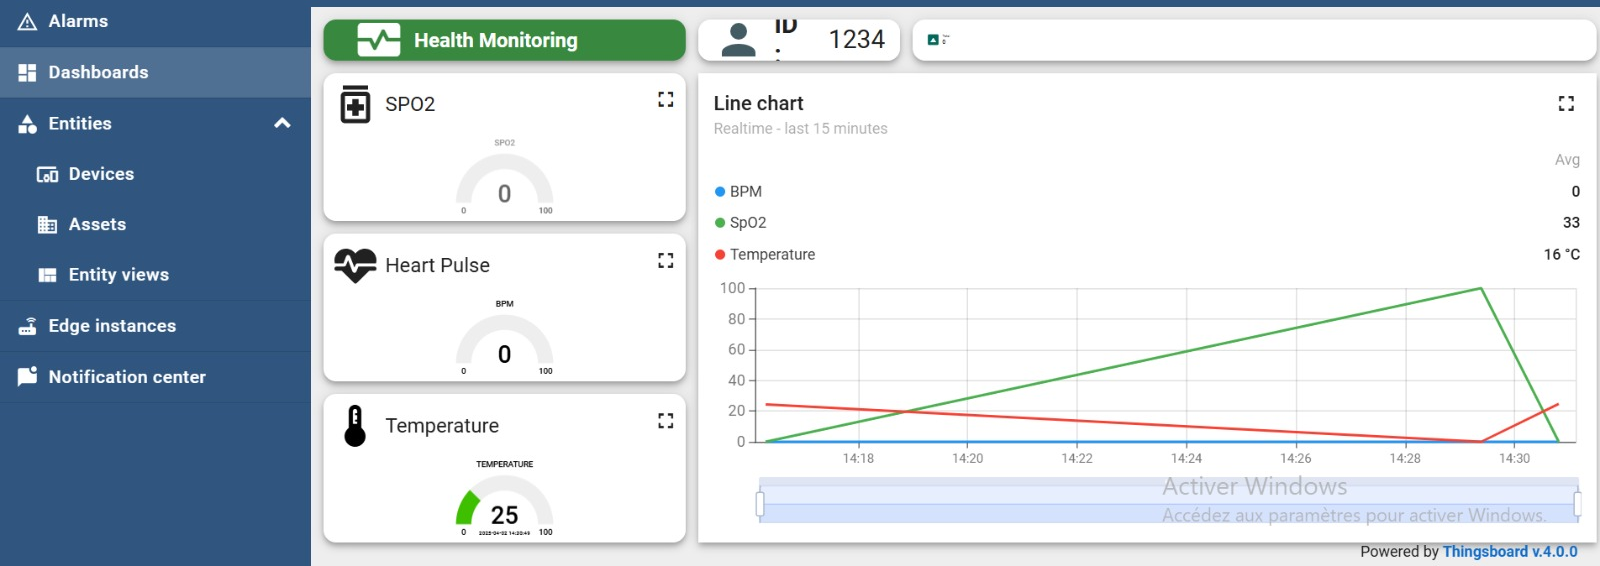
\includegraphics[width=0.8\linewidth]{images/fig-dashboard.png}
\caption{ThingsBoard patient-monitoring dashboard: live vital-sign
widgets and a rolling 15-minute line chart.}\label{fig:dashboard}
\end{figure}

\subsection{Why MQTT}

MQTT's fixed binary header (as small as 2 bytes) is an order of
magnitude smaller than HTTP's textual headers, and its
publish/subscribe model avoids the round-trip overhead of
polling-based protocols~\cite{mqtt311}. Quality-of-Service level 1
(``at least once'') is used for telemetry publishing, giving
guaranteed delivery without the duplicate-suppression overhead of
level 2.

\subsection{Topic Hierarchy}

Two MQTT paths are used in the system: the firmware publishes
combined telemetry to ThingsBoard's fixed ingestion topic
(\texttt{v1/devices/me/telemetry}, Listing~2); a second, per-vital
topic hierarchy on a public HiveMQ broker is used by the companion
Android application (Fig.~\ref{fig:hivemq-arch},
Sect.~\ref{sec:mobile}):
\begin{center}
\footnotesize\texttt{medmonitor/patient01/spo2},\ \texttt{medmonitor/patient01/hr},\ \texttt{medmonitor/patient01/temp}
\end{center}

\begin{figure}[!ht]
\centering
\resizebox{0.98\linewidth}{!}{%
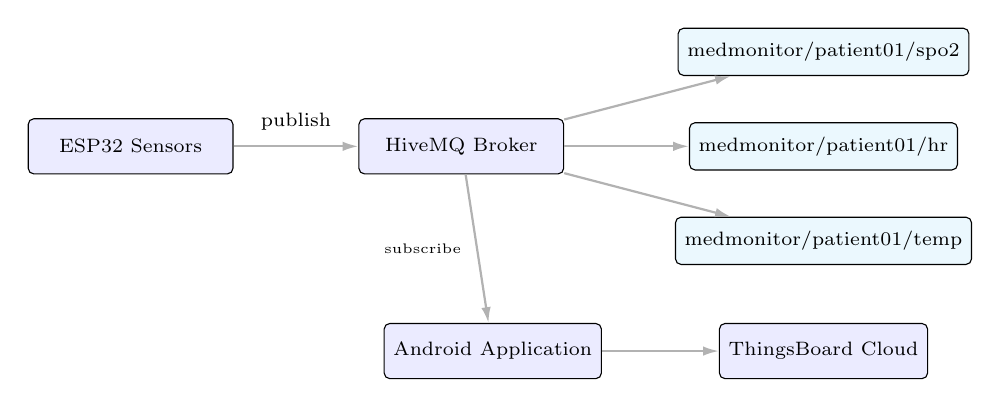
\begin{tikzpicture}[
  font=\scriptsize,
  every node/.style={align=center},
  box/.style={draw, rounded corners=2pt, fill=blue!8,
              minimum width=2.6cm, minimum height=0.7cm},
  topic/.style={draw, rounded corners=2pt, fill=cyan!8,
                minimum width=3.4cm, minimum height=0.6cm},
  arr/.style={-{Latex[length=2mm,width=1.2mm]}, thick, draw=gray!60}
]
\node[box] (esp) at (0,0) {ESP32 Sensors};
\node[box] (broker) at (4.2,0) {HiveMQ Broker};
\node[topic] (t1) at (8.8,1.2) {medmonitor/patient01/spo2};
\node[topic] (t2) at (8.8,0) {medmonitor/patient01/hr};
\node[topic] (t3) at (8.8,-1.2) {medmonitor/patient01/temp};
\node[box] (app) at (4.6,-2.6) {Android Application};
\node[box] (tb) at (8.8,-2.6) {ThingsBoard Cloud};

\draw[arr] (esp) -- node[above,yshift=2pt]{publish} (broker);
\draw[arr] (broker) -- (t1);
\draw[arr] (broker) -- (t2);
\draw[arr] (broker) -- (t3);
\draw[arr] (broker) -- node[left,xshift=-2pt,font=\tiny]{subscribe} (app);
\draw[arr] (app) -- (tb);
\end{tikzpicture}%
}
\caption{MQTT topic hierarchy for the Android companion application:
per-vital topics on a HiveMQ broker, subscribed to by the mobile app.}\label{fig:hivemq-arch}
\end{figure}

%%-----------------------------------------------------------------%%
\section{Mobile Application}\label{sec:mobile}

An Android companion application is under development as the primary
patient/clinician interface (Fig.~\ref{fig:androidapp}). Planned
features are: real-time vital-sign cards, a rolling historical chart,
threshold-based colour-coded alerts
(SpO\textsubscript{2}${}<{}$90\,\%, heart rate${}>{}$100\,bpm,
ambient temperature${}>{}$38\,$^\circ$C), and multi-patient profile
switching.
The application subscribes to the per-vital HiveMQ topics of
Fig.~\ref{fig:hivemq-arch}; during development, the broker's web
console confirmed three active topic subscriptions corresponding to
the SpO\textsubscript{2}, heart-rate, and temperature topics.

\begin{figure}[!ht]
\centering
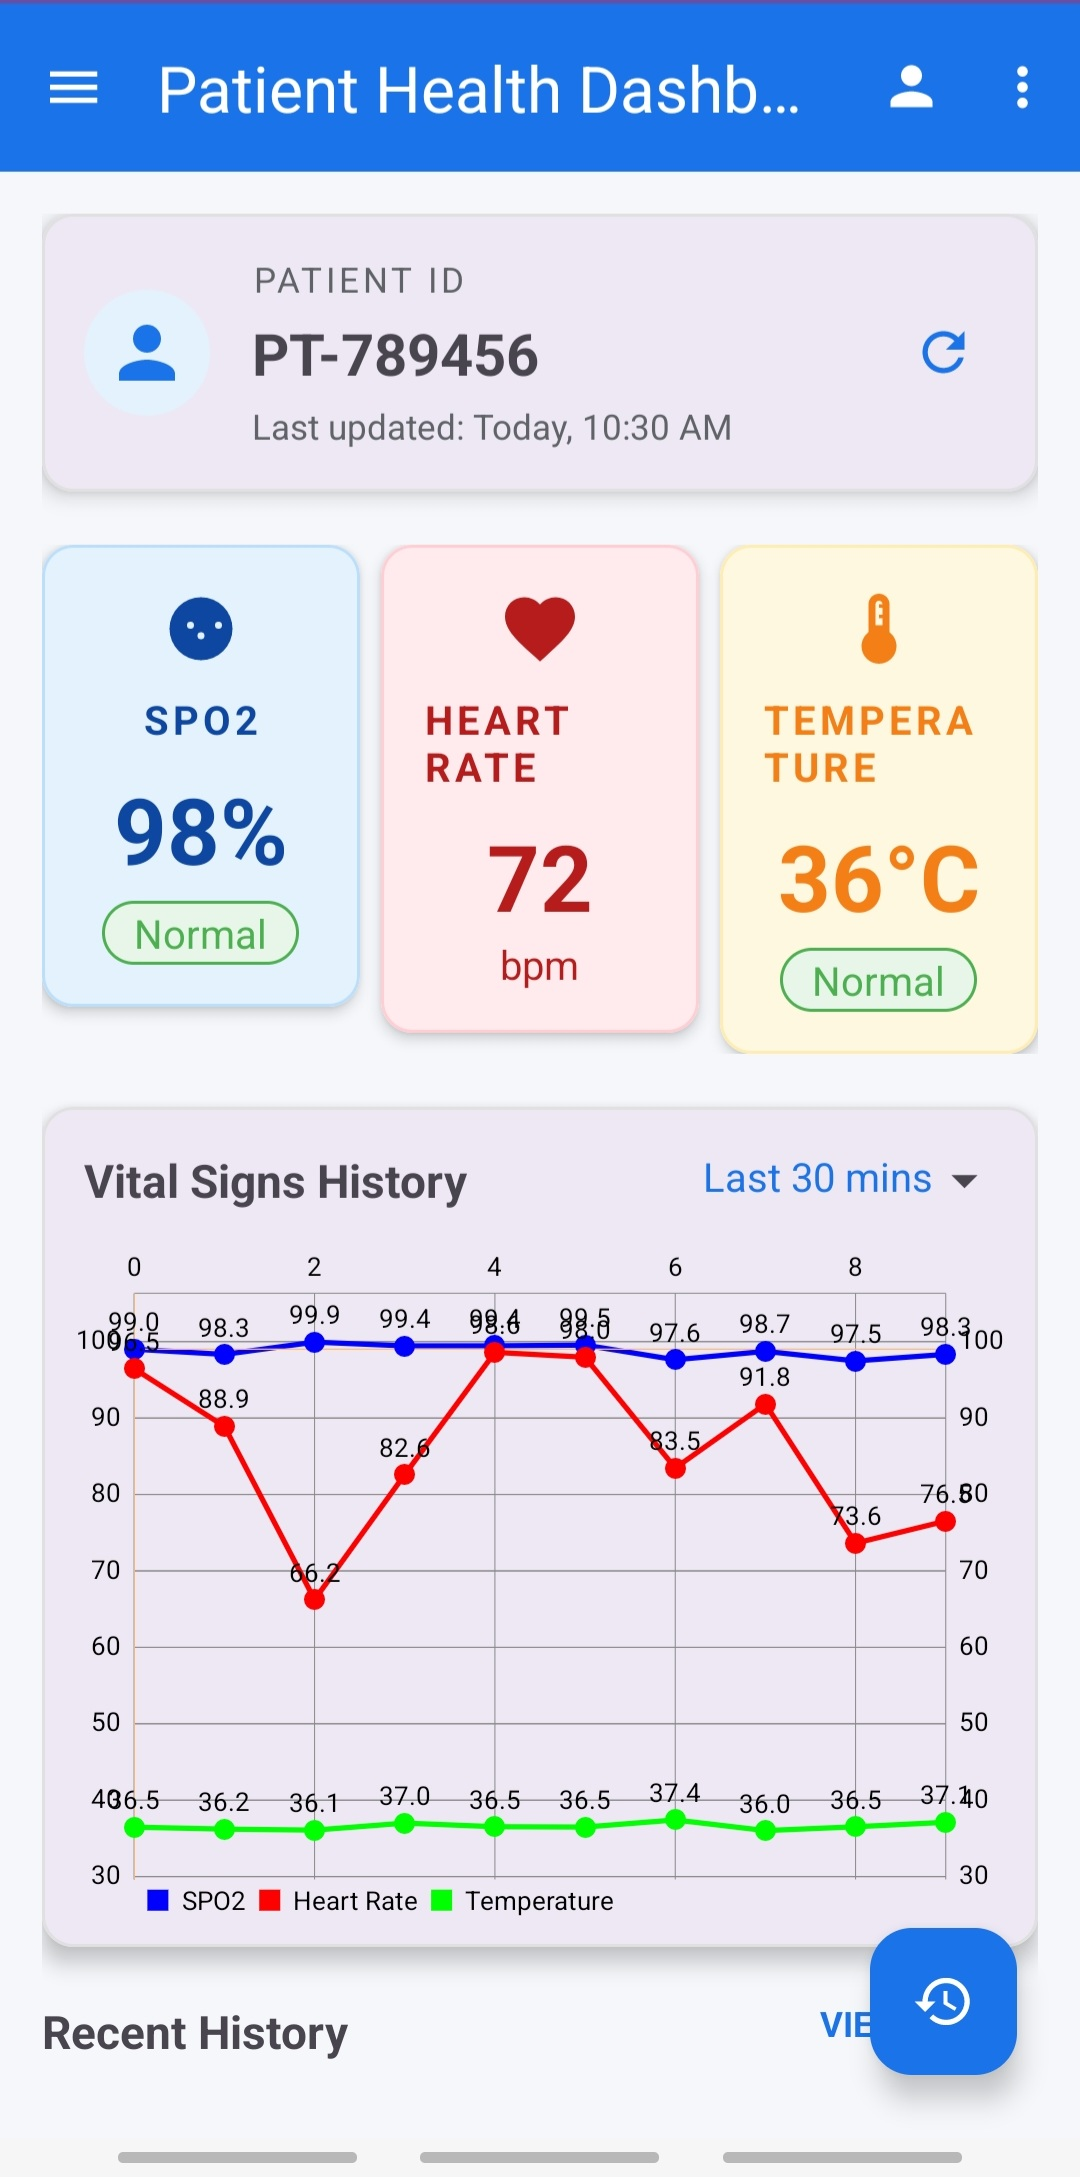
\includegraphics[width=0.38\linewidth]{images/fig-android-app.jpg}
\caption{Android application interface: vital-sign cards and a
30-minute history chart, captured live during a test session.}\label{fig:androidapp}
\end{figure}

%%-----------------------------------------------------------------%%
\section{Discussion}\label{sec:discussion}

Relative to the baseline of Gupta et al.~\cite{gupta2020}
(Table~\ref{tab:compare}), the prototype replaces an 8-bit
microcontroller with an integrated-wireless 32-bit dual-core ESP32,
replaces analogue LM35 thermometry with a digital DS18B20 probe
removing ADC quantisation noise, and replaces unencrypted HTTP
polling to a proprietary cloud service with MQTT publishing to an
open-source dashboard. The on-device patient-login menu adds a basic
access-control step absent from the baseline description.

\noindent\textbf{Limitations.} (i)~No clinical or statistical
validation of measurement accuracy against a reference instrument has
been performed; the system has been exercised on a single benchtop
prototype. (ii)~The demonstrated MQTT link uses the broker's default
unencrypted port for development, not the TLS listener intended for
production. (iii)~Blood-pressure sensing hardware is present on the
board design but not yet integrated into the firmware. (iv)~The
Android application has been exercised with live sensor data during
development but has not undergone formal usability evaluation with
patients or clinicians.

%%-----------------------------------------------------------------%%
\section{Future Perspectives}\label{sec:future}

Near-term work includes: (i)~clinical validation trials against a
reference vital-signs monitor at partner hospitals; (ii)~TLS-secured
production MQTT deployment (broker port 8883) with the same
token-based device authentication; (iii)~blood-pressure module
integration (HX711 load-cell front end) to complete the sensor set;
(iv)~portable ECG integration (AD8232
module); (v)~non-invasive glucose monitoring; (vi)~edge machine
learning for on-device anomaly detection; and (vii)~a voice
interface.

%%-----------------------------------------------------------------%%
\section{Conclusion}\label{sec:conclusion}

This paper presented an IoT-based healthcare monitoring prototype for
obese adults that improves on the platform of Gupta et
al.~\cite{gupta2020} through: (i)~MQTT-based telemetry in place of
unencrypted HTTP polling; (ii)~high-accuracy digital ambient-temperature
sensing (DS18B20, $\pm0.1\,^\circ$C); (iii)~a patient-authenticated
on-device interface feeding a JSON telemetry pipeline to an
open-source cloud dashboard; and (iv)~a concept design for a
multi-patient mobile dashboard with threshold-based alerting. Clinical
validation of measurement accuracy, TLS-secured production deployment,
and blood-pressure sensing integration are identified as near-term
future work.

\backmatter

\section*{Declarations}

\begin{itemize}
\item Funding: Not applicable.
\item Conflict of interest/Competing interests: The authors declare
  no competing interests.
\item Ethics approval and consent to participate: Not applicable;
  the study did not involve experiments on live vertebrates, higher
  invertebrates, human participants, or human samples.
\item Consent for publication: The individuals appearing in device
  photographs are members of the author team and have consented to
  the use of these images.
\item Data availability: Not applicable.
\item Materials availability: Not applicable.
\item Code availability: The ESP32 firmware source is available from
  the corresponding author upon reasonable request.
\item Author contribution: L.A., M.S., N.B., and M.D. carried out the
  hardware design, firmware development, and cloud integration; H.O.
  supervised the project and reviewed the manuscript. All authors
  read and approved the final manuscript.
\end{itemize}

%%-----------------------------------------------------------------%%
\begin{thebibliography}{7}

\bibitem{gupta2020}
Gupta,~D., Parikh,~A., Swarnalatha,~R.:
Integrated healthcare monitoring device for obese adults using
Internet of Things (IoT).
Int.\ J.\ Electr.\ Comput.\ Eng.\ \textbf{10}(2), 1239--1247 (2020).
\url{https://doi.org/10.11591/ijece.v10i2.pp1239-1247}

\bibitem{who2023}
World Health Organization: Obesity and overweight fact sheet.
WHO Press, Geneva (2023).
\url{https://www.who.int/news-room/fact-sheets/detail/obesity-and-overweight}

\bibitem{thingsboard}
ThingsBoard~Inc.: ThingsBoard Community Edition Documentation.
\url{https://thingsboard.io/docs/}

\bibitem{espressif}
Espressif Systems: ESP32 Series Datasheet.
Espressif Systems, Shanghai.

\bibitem{max30102ds}
Analog Devices (Maxim Integrated): MAX30102 High-Sensitivity Pulse
Oximeter and Heart-Rate Sensor Datasheet.

\bibitem{ds18b20ds}
Analog Devices (Maxim Integrated): DS18B20 Programmable Resolution
1-Wire Digital Thermometer Datasheet.

\bibitem{mqtt311}
OASIS: MQTT Version 3.1.1 Specification. OASIS Standard (2014).
\url{https://docs.oasis-open.org/mqtt/mqtt/v3.1.1/}

\end{thebibliography}

\end{document}
